\chapter{Introduction}	\label{ch:introduction}
%\glsresetall

\section{Introduction and state of the art.}
\subsection{Combustion}
\subsubsection{Premixed Flames(???)}
\subsubsection{Non-Premixed Flames}
\subsubsection{Droplet(?)}

%%%%%%%%%%%%%%%%%%%%%%%%%%%%%%%%%%%%%%%%%%%%%%%%%%%%%%%%%%%%%%%%%%%%%%%%%%%%%%%%%%%%%%%%%%%%%%%%%%%%%%%%%%%%%%%%%%%%%%%%%%%%%%%%%%%%%%%%%%%%%%%%%%%%%%%%%%%%

%\textcite{leeTwodimensionalDirectNumerical2000} paper donde hablan de comparacion entre quasi one-dimensional and two-dimensional  counter diffusion flame
High order discretization methods is a topic which has been gaining increasing attention in the last decades. An important exponent of them is the Discontinuous Galerkin (DG) method \textcite{cockburnDevelopmentDiscontinuousGalerkin2000}. The DG method was initially developed and utilized for solving hyperbolic conservation laws, especially in the field of computational fluid dynamics (CFD), and has recently gained increased attention for incompressible CFD problems for structured and unstructured grids. Two main advantages stand out when compared with traditional methods such as the Finite Volume Method (FVM) or the Finite Difference Method (FDM): First, DG offers an arbitrary order of error convergence due to the polynomial local approximation of the solution field. A polynomial approximation of degree $p$ provides a numerical discretization error of the order  $\mathcal{O}(h^{p+1})$ for sufficiently smooth solutions, where $h$ is a characteristic grid length.
Secondly, regardless of the desired order of accuracy, any given cell of the grid only requires information from its immediate neighbours, allowing for efficient parallelization with minimal communication overhead. In contrast, more traditional schemes, such as the FVM, are usually limited to $\mathcal{O}(h^N)$ accuracy, with $N \leq 2$ for unstructured grids. Even for structured grids $N$ is practically limited to low values due to the increasing stencil size for increasing $N$. Advantageously the DG method offers the locality of low-order schemes and the accuracy per degree of freedom of spectral schemes.

In the context of CFD solvers, an important distinction is that between pressure-based and density-based solvers. Historically, pressure-based solvers have been used for incompressible flows, i.e. flows with divergence-free velocity fields. On the other hand, density-based (also called fully compressible) solvers should, in theory, be able to solve flows in all Mach number ranges. However, in practice, as the Mach number approaches zero, density-based solvers experience efficiency and accuracy problems. These issues are mainly attributed to the acoustic effects in the flow, which tends to generate very stiff systems. None of these approaches are directly applicable to flows with varying density in the low-Mach limit. \textcite{henninkPressurebasedSolverLowMach2021} It is possible, however, to extend existing incompressible and compressible codes so that they are capable of dealing with low Mach numbers. \textcite{keshtibanCompressibleFlowSolvers2003} In this work a extension from a incompressible solver is presented.

There are numerous works in which the DG method has been used within the context of incompressible flows. \textcite{shahbaziHighorderDiscontinuousGalerkin2007,kummerBoSSSDiscontinuousGalerkin2012,kleinSIMPLEBasedDiscontinuous2013,rhebergenSpaceTimeDiscontinuous2013}  However, there are not many publications in which the flow problem at low Mach numbers is addressed using a pressure-based solver. In the work by Klein et al. \textcite{kleinHighorderDiscontinuousGalerkin2016} the low-Mach equations are solved in a DG Framework making use of a SIMPLE type scheme. The solution of a time-step involves an iterative process that requires multiple matrix assemblies and solutions. The obtained systems of equations are solved by means of fixed-point iterations, where relaxation factors are necessary to obtain convergence of the computations.
In the work of Hennink et al. \textcite{henninkPressurebasedSolverLowMach2021} a pressure-based solver for low-mach flows is presented. They solve  the mass flux instead of the velocity as the primitive variable.

High order methods are very attractive for complex reacting fluid dynamical systems, where usually a high numerical resolution is necessary. Particularly for combustion problems, where large amounts of heat are released in rather small zones within the flow, the high number of elements required to resolve the resulting steep gradients could result in prohibitive calculation times even for simple problems. In particular the study of so-called diffusion flames -- also known as non-premixed flames -- requires special consideration. In a diffusion flame, the reactants are initially spatially separated. For this kind of system, mixing plays a crucial role because reactants need to be brought together to the flame zone in order to maintain combustion. Many practical applications of diffusion flames consider deflagration flames, \textcite{poinsotTheoreticalNumericalCombustion2005} which are characterized by a small characteristic velocity compared to the speed of sound. The low-Mach approximation of the Navier--Stokes equations is often chosen for describing this kind of system. This approximation allows for the calculation of non-constant density flows (such as temperature dependent density), while neglecting acoustic effects, thus dramatically reducing the required temporal resolution. \textcite{mullerLowMachNumberAsymptoticsNavierStokes1998}

In addition to the compressibility effects mentioned above, the need to accurately and efficiently represent the chemical reactions governing the combustion problem poses a major challenge. Generally speaking, to study the combustion process a detailed chemistry description is preferable. However, this is often impractical as it can be very intensive computationally speaking. Stauch et al. investigated systems with detailed mechanism for methanol combustion, where 23 chemical species and 166 elementary reactions are involved, \textcite{stauchDetailedNumericalSimulation2006} and for n-heptane with 62 chemical species and 572 elementary reactions, and with detailed transport processes\textcite{stauchAutoignitionSingleNheptane2007}. Because of their high complexity the mentioned works are restricted to simple one- or two-dimensional configurations, and to a small number of grid elements. If one is interested in more complex geometries or more complicated flow systems, the use of detailed kinetics can be prohibitive. Simplified kinetic models have been developed to overcome this difficulty. In the work of Westbrook et al. \textcite{westbrookSimplifiedReactionMechanisms1981} a one-step kinetic model is presented, where combustion is expressed as a single chemical reaction with a reaction rate given by an Arrhenius-type expression with constant parameters. Multi-step chemical reaction models have also been developed, such as the four-step mechanism for methane combustion by Peters, \textcite{petersNumericalAsymptoticAnalysis1985} or the three-step mechanism by Peters and Williams. \textcite{petersAsymptoticStructureStoichiometric1987}
Furthermore, extensions of one-step models exist, such as the one presented by Fernandez-Tarrazo et al. \textcite{fernandez-tarrazoSimpleOnestepChemistry2006} for hydrocarbon combustion with air, where kinetic parameters are correlated to the equivalence ratio in order to better describe characteristic flame properties for premixed and non-premixed flames.

In the last decades several numerical investigations related to diffusion flames have been carried out. Burke and Schumann were the first ones to investigate the structure of diffusion flames by studying the flame jet problem. \textcite{burkeDiffusionFlames1928} By assuming an infinitely fast chemical reaction they managed to predict flame properties fairly accurately. In the work of Smooke et al. \textcite{smookeNumericalSolutionTwoDimensional1986} a numerical simulation for a two-dimensional axisymmetric laminar diffusion jet  with detailed chemistry was conducted and solved with Newton-type methods. In order to obtain adequate initial estimates for this problem, the solution of the problem for an infinitely fast chemistry was solved first. This idea was used in several works such as that by Keyes and Smooke \textcite{keyesFlameSheetStarting1987} for a counter diffusion flame, by Smooke \textcite{smookeNumericalModelingAxisymmetric1992} for a Tsuji-counterflow configuration and in the work by Dobbins et al. \textcite{dobbinsFullyImplicitCompact2010} for an axisymmetric laminar jet diffusion flame with time dependent boundary conditions. In the work of Paxion \textcite{paxionDevelopmentParallelUnstructured2001} unstructured multigrid solver for laminar flames with detailed chemistry is presented. A Krylov-Newton method was used for solving several flame configurations. A two-dimensional counter diffusion flame was calculated, and its results were compared with the one-dimensional self-similar solution of the equations.

The DG method has also been used for simulations of combustion, mainly within a fully compressible framework. In the work from Johnson et al. \textcite{johnsonConservativeDiscontinuousGalerkin2020} the compressible Navier--Stokes equations are solved using a nodal DG scheme for combustion with complex chemistry and transport parameters. An hp-adaptive method is also presented, and shown to be useful for solving the ordinary differential equations used for describing the unsteady behaviour of the system.  Similarly in the work from Lv and Ihme \textcite{lvHighorderDiscontinuousGalerkin2017} a DG solver for multi-component chemically reacting flows, which solves the fully compressible Navier-Stokes equation, is presented. A hybrid-flux formulation is used, where a conservative Riemann solver is used for shock treatment, and a double-flux formulation is used in smooth regions. They show its applicability for non-reacting and reacting flows, particularly for systems characterized by high Mach numbers. On the other hand, the solution of combustion problems using the DG method in an incompressible framework is a topic that has not received much attention in the literature. This fact is the motivation of the present paper.

The system of equations obtained from the discretization of highly nonlinear systems  can be very difficult to solve. Fixed-point iteration schemes have been used as a linearization strategy, as done by Klein et al. \textcite{kleinHighorderDiscontinuousGalerkin2016} A major drawback of this approach is the highly problem dependent choice of under-relaxation factors. A much more robust strategy is the use of Newton type methods. \textcite{shadidInexactNewtonMethod1997,pawlowskiGlobalizationTechniquesNewton2006} Here, a problem-dependent factor is not needed. There is however a trade-off, because the Jacobian matrix has to be calculated, which can be computationally expensive. This approach has been used for combustion problems in numerous works. Karaa et al. \textcite{karaaPreconditionedMultigridSimulation2003} studied the axisymmetric laminar jet diffusion flame and investigated the behaviour of a multi-grid solver when using different pre-conditioners with a damped Newton algorithm. Shen et al. \textcite{shenNewtonMethodSteady2006a} investigated the use  and efficiency of a Newton method coupled with the Bi-CGSTAB method for an axisymmetric laminar jet flame. They concluded that, in terms of computational cost, the steady-state solution  is more efficiently obtained by directly solving the steady formulation of the equations, than by solving the transient Navier-Stokes equations until the steady state is reached.

It is well known that the Newton method shows the property of having quadratic convergence sufficiently close to the solution\textcite{deuflhardNewtonMethodsNonlinear2011}. However, if the initial solution guess is not adequate, the method converge to a solution slowly, or may not even converge at all. For some highly nonlinear problems this is a significant issue. The so-called globalized Newton methods are used to overcome this problem by effectively increasing the area of convergence of the method. A popular globalized Newton method is the Newton-Dogleg method, \textcite{pawlowskiInexactNewtonDogleg2008} which is based on a trust-region technique.

In the present work, a steady low-Mach pressure-based solver for the simulation of temperature dependent non-reactive and reactive flows using the Discontinuous Galerkin method is presented.
To the best of our knowledge, this is the first time that a pressure-based solver is used together with the DG method for solving the reactive low-Mach equations using the Newton-Dogleg method in a fully coupled manner. We focus in this study on two-dimensional configurations, but the ideas presented could be extended to three-dimensional systems. The one-step combustion model presented by Fernandez-Tarrazo et al. \textcite{fernandez-tarrazoSimpleOnestepChemistry2006} is used for describing the chemical reactions. In the present work we consider only methane combustion, but the one-step model could be used for other hydrocarbons as well. We choose this chemical model to obtain physically correct results for a wide range of applications, while avoiding the use of complex chemistry models. The discrete system of equations is solved by a globalized Newton method, by means of the Dogleg approach. In addition to the Newton-Dogleg method, a homotopy strategy is presented, which was found to be useful for obtaining solutions of steady state calculations of highly nonlinear problems. In order to find appropriate initial values for Newton's method in combustion applications, the concept of flame sheet estimates (i.e. the solution for infinitely fast chemistry) is used. Several benchmark cases are presented that allow us to validate our implementation. First we solve the differentially heated cavity problem, with which we intend to validate our implementation of the low-Mach solver for non-constant density flows using the fully coupled solver. Later two flame configurations are calculated, namely the counter-diffusion flame and the chambered diffusion flame. \parencite{matalonDiffusionFlamesChamber1980}

In the following, we consider a two-dimensional system. However, the methods shown in this work could be also used for three-dimensional problems.
%%%%%%%%%%%%%%%%%%%%%%%%%%%%%%%%%%%%%%%%%%%%%%%%%%%%%%%%%%%%%%%%%%%%%%%%%%%%%%%%%%%%%%%%%%%%%%%%%%%%%%%%%%%%%%%%%%%%%%%%%%%%%%%%%%%%%%%%%%%%%%%%%%%%%%%%%%%%%%%%%%%%%%%%%%%%%%%%%%%%%%%%%%%%%%%%%%%%

% hablar sobre la derivacion (historica) de las ecuaciones de low mach. Porque son utiles? 
They were first derived by Rehm and Baum \parencite{rehmEquationsMotionThermally1978}. A rigorous extension to combustion problems was done by Majda and Sethian \parencite{majdaDerivationNumericalSolution1985}.



\textcite{pitschConsistentFlameletFormulation1998} Habla sobre pposibles formas de escribir las ecuaciones para un flamelet de tal forma que sea posible contabilizar la diffusion diferencial (non unity lewis numbers.)


%Conservative High-Order Finite Difference
%Schemes for Low-Mach Number Flows
%F. Nicoud 1
%owever, for the particular class of flow with
%low Mach number M and strong density variation, the classical compressible Navier-Stokes equations are not well suited for computation. The small
%time step limitation dictated by numerical stability requirements of explicit
%methods would require excessive computing times to solve practical flow
%problems. Indeed the sound waves move much faster than entropy or vorticity waves when M << 1. At the same time, in flows where the dominating
%mechanism is free, forced or mixed convection, the acoustical mode of energy
%carries only a small fraction of the energy present in the fluctuating part of
%the flow. These observations led several authors [1, 2, 3, 4] to propose a set
%of low-Mach number equations which do not contain acoustic waves but can
%still describe the entropy and vorticity modes as well as compressibility due
%to exothermicity of chemical reactions. A fractional-step method is used
%most often, the pressure field being obtained by solving a Poisson equation
%with the time derivative of the density field as part of the source term [3, 5].


%% Esto viene de la discusion de resultados: ya lo quite de ahi, asi que hay que ponerlo aca
%%% It was also observed that the calculation times were prohibitively high for some test cases. This point motivated the development of the solver presented in the present work, where the system is solved in a monolytic way and  and the Newton method globalized with a Dogleg-type method is used to solve the system.

% En la introduccion deberia dar una motivacion de porque esto es asi y porque se creó el solver fully coupled sin SIMPLE
%TODO \todo[inline]{what are exactly the advantages of the present solver? multigrid? Ortogonalization?} 

\subsection{The \gls{BoSSS} code}
The presented solver is embedded in the \textit{BoSSS} (Bounded Support Spectral Solver) code, which is under active development at the chair of fluid dynamics of the Technical University of Darmstadt, and is available under \href{https://github.com/FDYdarmstadt/BoSSS}{https://github.com/FDYdarmstadt/BoSSS}.

\BoSSS is a general framework for the discretization of conservation laws using the DG method and uses a modal DG approach with orthonormal Legendre polynomials as basis functions. The \BoSSS code features a variety of applications in the context of computational fluid dynamics, such as a solver for multiphase flows with a sharp interface approach, \parencite{kummerExtendedDiscontinuousGalerkin2017} an incompressible Immersed Boundary Method solver for particle laden flows,\parencite{krauseIncompressibleImmersedBoundary2017} a solver for viscoelastic fluid flows,\parencite{kikkerFullyCoupledHighorder} and a solver for compressible flows, \parencite{geisenhoferDiscontinuousGalerkinImmersed2019} among others.



From this point on, the solver presented in this work will be called XNSEC (e\textbf{X}tended \textbf{N}avier-\textbf{S}tokes for \textbf{C}ombustion). The term \textit{extended} refers to the framework on which the solver is built, which focuses on applications for multi-phase flows using a sharp interface approach using a level-set method. This point will be briefly discussed in the section %TODO future work chapter
\begin{figure}
	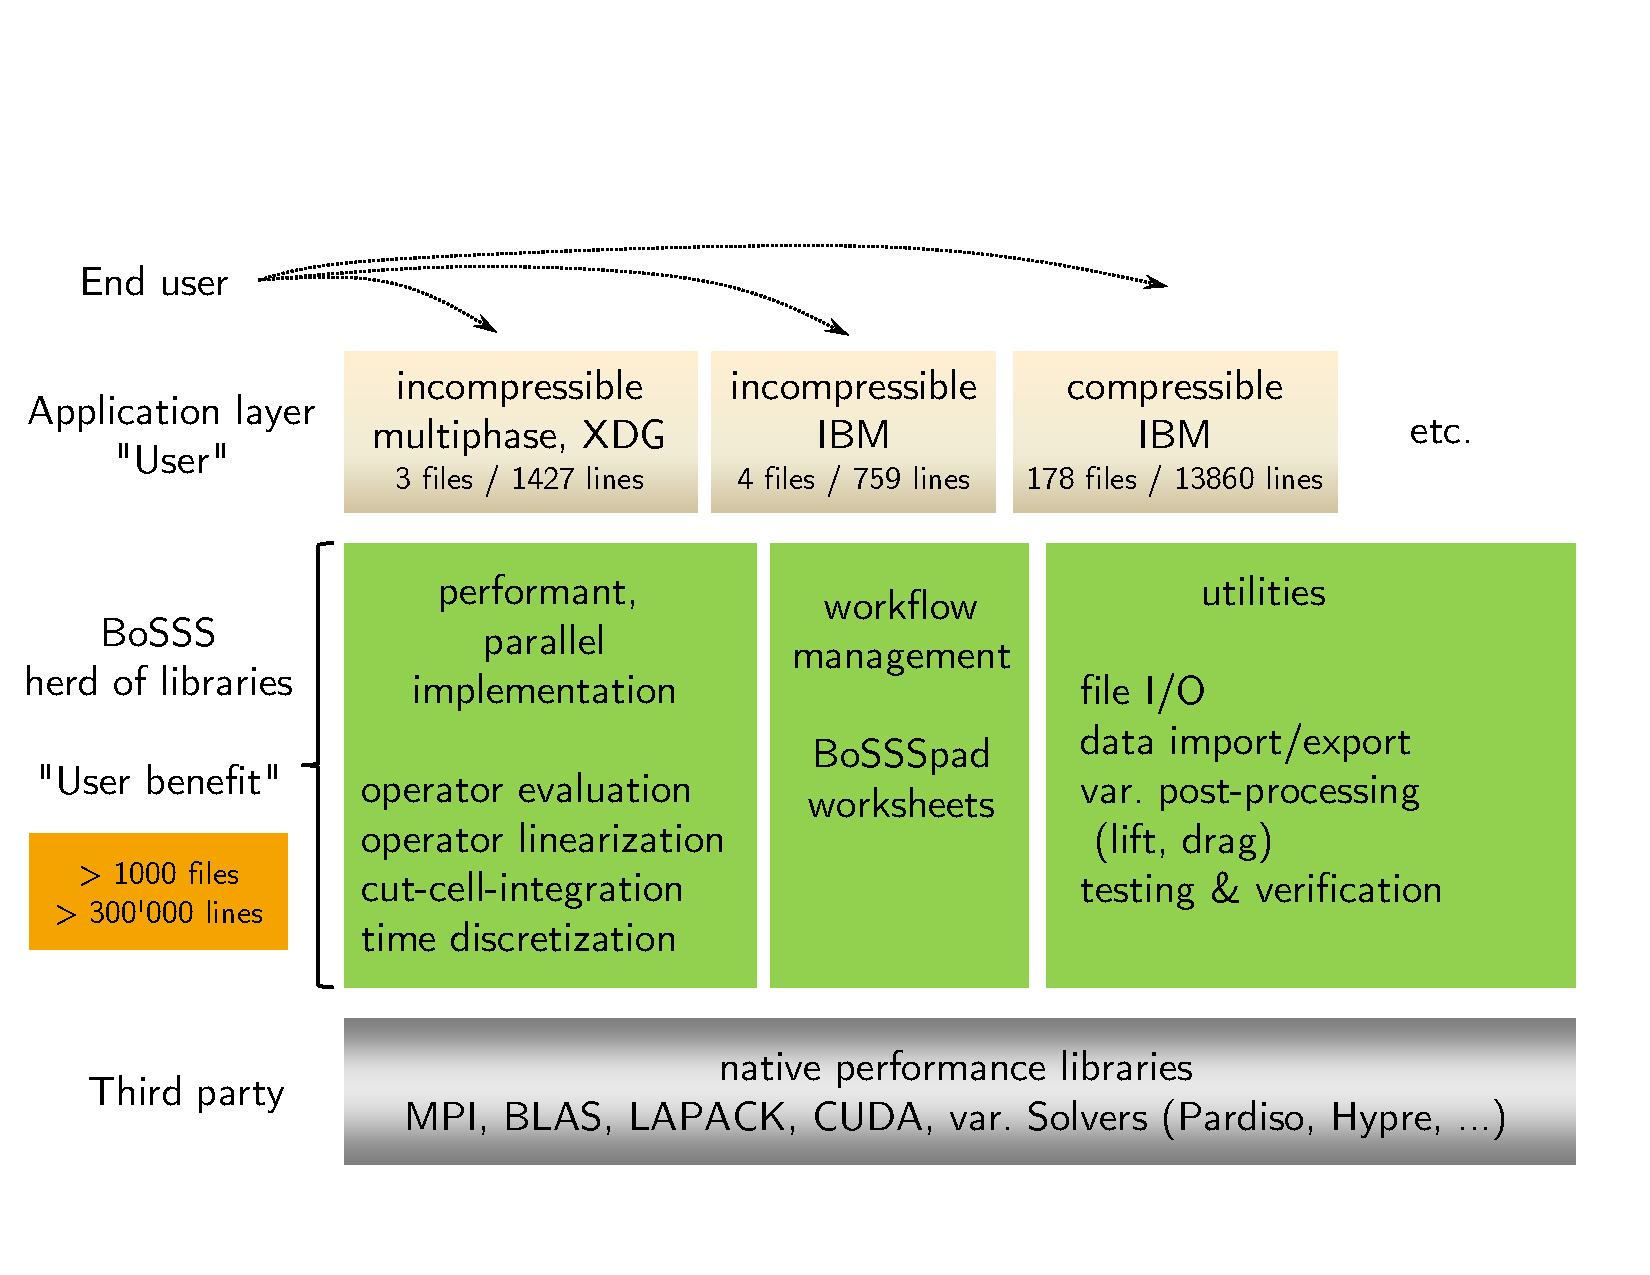
\includegraphics[width=\textwidth]{BoSSS-philosophy-1.pdf}
	\caption{Schematic representation of the estructure of the \gls{BoSSS} solver from the \gls{BoSSS} handbook \parencite{kummer2020}.}
	\label{Fig:BoSSS}
\end{figure}


\subsection{Motivation and objectives of this work}
two-dimensional 